% !TeX TXS-program:compile = txs:///pdflatex/[--shell-escape]

\documentclass[11pt, letterpaper]{article}

\usepackage{minted}
\usepackage[utf8]{inputenc}
\usepackage[T1]{fontenc}
\usepackage{lmodern}
\usepackage{graphicx}
\usepackage{longtable}
\usepackage{wrapfig}
\usepackage{rotating}
\usepackage{amsmath}
\usepackage{textcomp}
\usepackage{amssymb}
\usepackage{hyperref}
\usepackage[round]{natbib}
\usepackage{subcaption}


\title{\bfseries Tarea}
\author{Ángel García Báez}
\date{\today}
\setcounter{tocdepth}{3} 

\begin{document}
	
	% Página de presentación
	\begin{titlepage}
		\centering
		
\includegraphics[width=0.2\textwidth]{logo.png}\par
		\vspace{1cm}
		{\LARGE \bfseries Universidad Veracruzana \par}
		\vspace{1cm}
		{\Large Maestría en Inteligencia Artificial\par}
		\vspace{3cm}
		{\LARGE \bfseries Visión por Computadora \par}
		\vspace{1cm}
		{\Large \bfseries Tarea 5. Aplicación de PCA a la base de datos de pingüinos palmer en MATLAB. \par}
		\vfill
		{\Large \textit{Ángel García Báez}\par}
		\vspace{1cm}
		{\Large Profesor: Dr. Héctor Acosta Mesa y Dra. Adriana Laura López Lobato\par}
		\vfill
		{\Large \today \par}
	\end{titlepage}
	
	% Página exclusiva para la tabla de contenidos
	\newpage
	\tableofcontents
	\newpage
	
% Sección para el problema 1
\section{Objetivo de la práctica}
	
Se tiene la base de datos de pingüinos palmer, la cual representa las mediciones de 3 especies de pingüinos en distintas islas, a lo largo de distintos años, la cual tiene la siguiente estructura:




\begin{figure}[h!]
	\centering
	\begin{minipage}{1\textwidth}
		\centering
		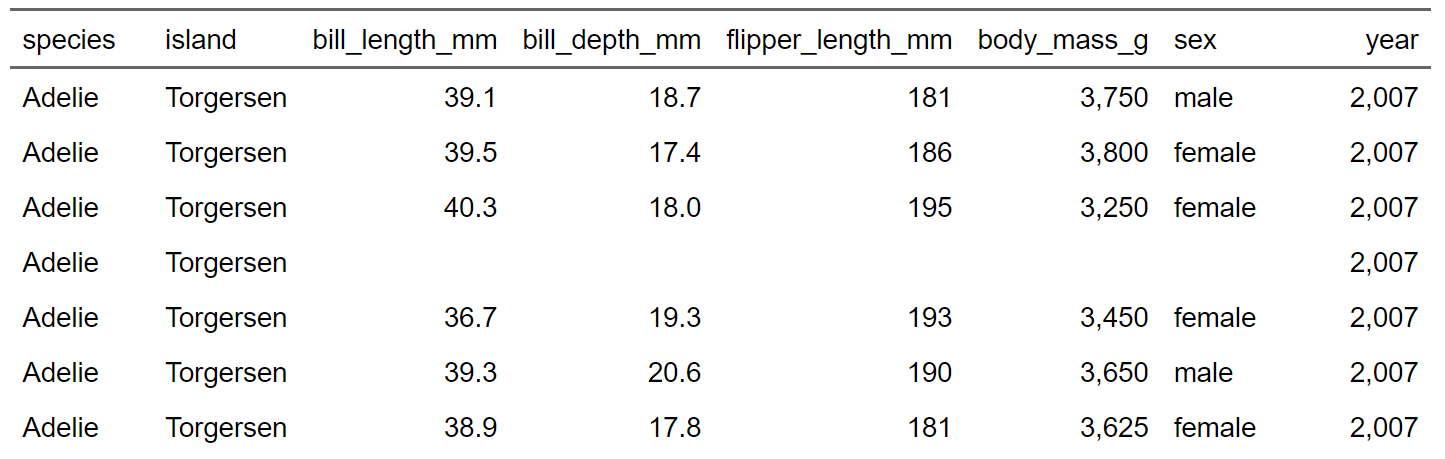
\includegraphics[width=\textwidth]{IMG/T1.png}
		\caption{Base de datos de los pingüinos palmer (primeros 5 casos)}
		\label{fig:f1}
	\end{minipage}\hfill
\end{figure}

La base esta compuesta por 344 observaciones y 8 variables (4 variables categóricas o de etiqueta y 4 variables numéricas continuas). Para efectos del desarrollo del documento, se tomaran en cuenta unicamente las 4 variables numéricas continuas (bill\_length, bill\_depth, flipper\_length y body\_mass) junto con la variable categórica de species para hacer el coloreado en los gráficos.


\newpage

La problemática que se desea abordar y  por la cual se quiere aplicar PCA es la siguiente: Se desea poder proyectar la información de las 4 dimensiones en un espacio de menor dimensionalidad, esto con la finalidad de poder observar gráficamente como se están comportando los datos.

A continuación se muestran aproximaciones en 2D mediante gráficos de dispersión entre las variables, con el objetivo de evidenciar lo difícil que es ver como se están comportando los datos:


\begin{figure}[h!]
	\centering
	\begin{minipage}{1.1\textwidth}
		\centering
		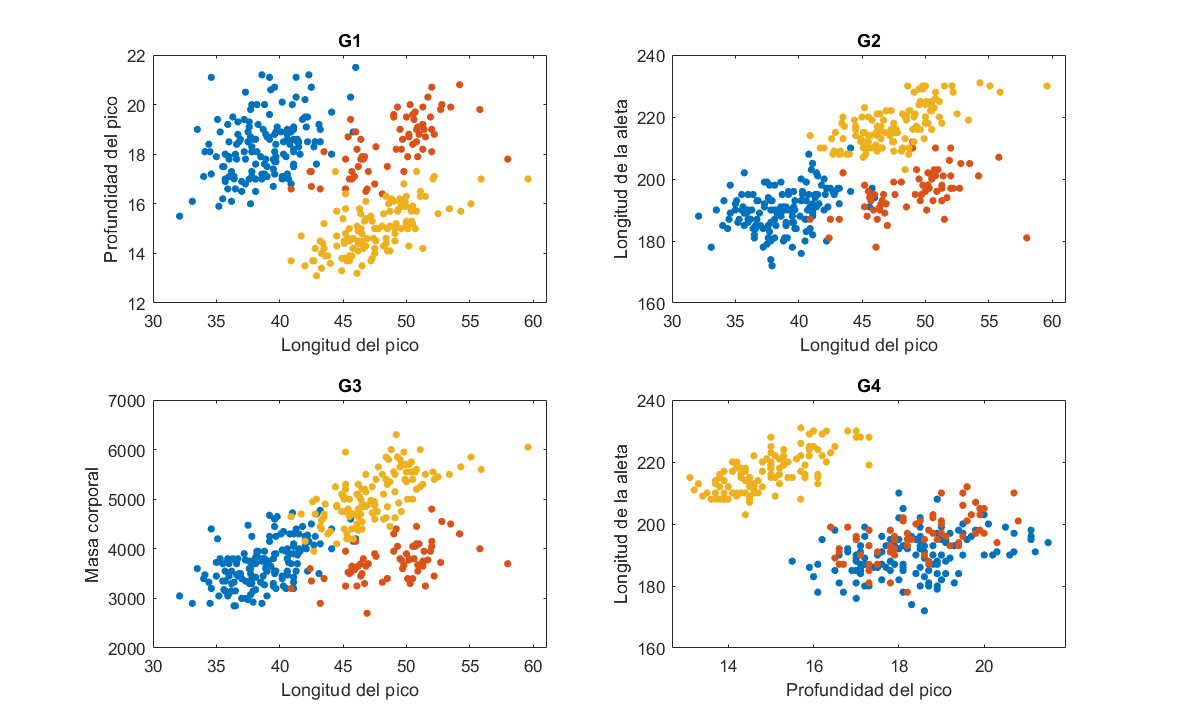
\includegraphics[width=\textwidth]{IMG/G1.png}
		\caption{Gráficos de dispersión bivariados.}
		\label{fig:f2}
	\end{minipage}\hfill
\end{figure}

Se puede observar que para algunos pares de variables, se alcanza a ver una separación clara de los datos por especies, sin embargo, al verlo desde otro par de variables, la cosa se vuelve difusa de distinguir, como es el caso del gráfico G4, en donde se esta mostrando el comportamiento de las variables de la profundidad del pico y el largo de la aleta.

\newpage

Por otro lado, se hizo la propuesta de modelarlos en 3 dimensiones, para observar como se comportan los datos en el espacio:

\begin{figure}[h!]
	\centering
	\begin{minipage}{1.1\textwidth}
		\centering
		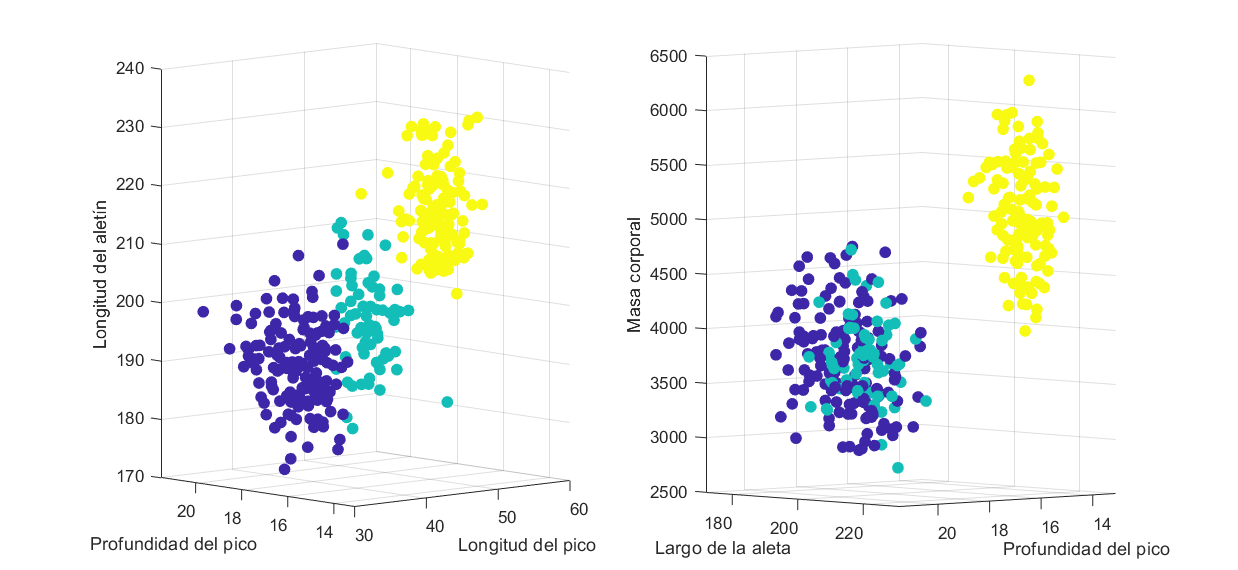
\includegraphics[width=\textwidth]{IMG/G2.png}
		\caption{Gráficos de dispersión multivariados.}
		\label{fig:f3}
	\end{minipage}\hfill
\end{figure}


En el primer gráfico se logra apreciar una separación distinguible entre los grupos de pingüinos dada su visualización mediante las variables de profundidad del pico, longitud del pico y longitud de la aleta. Por otro lado, en el gráfico de la derecha, se observa como un grupo esta perfectamente diferenciado del resto pero los 2 grupos restantes se encuentran sobre puestos uno con el otro, lo que los hace difíciles de separar usando las variables de profundidad del pico, largo de la aleta y masa corporal.

Es por ello que se quiere usar PCA para comprimir la información y reducir la dimensionalidad de los datos para proyectarlos en un espacio de menor dimensión y observar mejor su comportamiento en 2 y 3 dimensiones.

	
	\newpage
	
	\section{Metodología}
	
	Para realizar el calculo del PCA es necesario desglosarlo en varios pasos. Primero, cabe mencionar que el PCA es una técnica multivariada de aprendizaje no supervisado que permite reducir la dimensionalidad de datos cuantitativos continuos al proyectar la información en un nuevo espacio de variables incorrelacionadas sin perder apenas información en la transformación como se explica en el libro de \cite{johnson2007}. 
	
	Para ejecutar la técnica, se sugiere primero obtener el vector de medias de la matriz y restarselo a la misma para centrar los datos y garantizar que el subespacio vectorial que va a encontrar la técnica contiene al vector nulo $\vec{0}$ como se muestra a continuación:
	
	$$
	 \begin{matrix}
	 	X = \{x_1,x_2,\dots,x_n\} \\
	 	 \bar{X} = \{\bar{x}_1,\bar{x}_2,\dots,\bar{x}_n\} \\
	 	X_c = X-\bar{X}
	 \end{matrix}
	$$
	Donde: 
	\begin{itemize}
		\item $X$ es la matriz de datos de tamaño $N\times P$.
		\item $\bar{X}$ Es el vector de medias de tamaño $1\times P$.
		\item $X_c$ Es la matriz de datos centrados en la media.
	\end{itemize}
	
	Una vez que se tiene la matriz centrada, se procede con el calculo de su matriz de varianzas y covarianzas como sigue:
	
	$$S = \frac{1}{n-1} (X-\bar{X})' (X-\bar{X})$$
	
	Donde: 
	\begin{itemize}
		\item $X$ es la matriz de datos de tamaño $N\times P$.
		\item $\bar{X}$ Es el vector de medias de tamaño $1\times P$.
		\item $N$ Es la cantidad de observaciones en la matriz X.
	\end{itemize}

\newpage

Una vez que se tiene lista la matriz de covarianzas, es necesario descomponerla en sus valores y vectores propios (eigen valores y eigen vectores) para encontrar el nuevo espacio donde proyectar los datos originales. Para esto se plantea la siguiente ecuación característica sobre la matriz de varianzas y covarianzas:

$$Sv = \lambda v$$

	Donde: 
	\begin{itemize}
		\item $S$ es la matriz de varianzas y covarianzas de los datos de tamaño $P\times P$.
		\item $\lambda$ son los valores propios asociados a la matriz.
		\item $v$ son los vectores propios asociados a la matriz .
	\end{itemize}

Haciendo un pequeño arreglo, se reescribe la ecuación y queda tal que así:

$$
\begin{matrix}
Sv-\lambda v = 0 \\
(S-\lambda I_P)v = 0	
\end{matrix}
$$

Posterior a ello, se procede con la resolución del sistema de ecuaciones para hallar los valores propios ($\lambda$) y los vectores propios $v_i$ donde cabe recalcar que se pone la restricción de que las componentes al cuadrado del $i$-ésimo vector propio deben sumar 1.

El resultado esperado son $P$ valores propios que indican cuanta varianza acumula cada una de las componentes en el nuevo sistema de coordenadas donde se van a proyectar los datos originales y $P$ vectores propios que serán los ejes sobre los cuales se proyecten los datos y construyan las nuevas componentes donde los datos proyectados tendrán la particularidad de ser incorrelacionados.

Para hacer la proyección de los datos centrados en el nuevo sistema, basta con aplicar la siguiente operación matricial con los vectores propios encontrados:

$$Z = X_cv$$

Donde: 
\begin{itemize}
	\item $Z$ Son los componentes creados a partir de los datos centrados y los vectores propios.
	\item $X_c$ Es la matriz de datos centrados de tamaño $N \times P$.
	\item $v$ es la matriz de vectores propios de tamaño $P \times P$ .
\end{itemize}

Finalmente, se calcula la variabilidad explicada por cada componente mediante los valores propios como sigue:

$$VE = 100*\frac{\lambda_i}{\sum_{i = 1}^P{\lambda_i}}$$

Donde: 
\begin{itemize}
	\item $VE$ Es la variabilidad explicada por el $i$-ésimo valor propio.
	\item $\lambda_i$ Es el $i$-ésimo valor propio.
\end{itemize}

Cabe mencionar que los valores propios conservan la siguiente propiedad:

$$\lambda_1 \geq \lambda_2 \geq \dots \geq \lambda_P$$

El primer valor propio es mayor o igual al segundo valor propio, el segundo es mayor o igual al tercer y así sucesivamente. El primer valor propio asociado a la primer componente siempre sera el que mayor variabilidad explique (asumiendo que están ordenados de mayor a menor, esto ya es tema de notación y en que orden se realicen las operaciones de matrices).

A continuación se aplicara la PCA para reducir dimensionalidad sobre la base de datos de pingüinos palmer calculando el vector de medias, la matriz centrada, los valores propios, los vectores propios y realizando la visualización de los componentes en 2 y 3 dimensiones.
	
\newpage
	
\section{Resultados}

A continuación se muestran los resultados obtenidos para los datos de los pingüinos palmer en matlab.

\subsection{Vector de medias}

Se muestra el vector de medias obtenido para las variables de Longitud del pico, profundidad del pico, longitud de la aleta y la masa corporal:

$$\bar{X} = \{43.92,\quad 17.15,\quad  200.91,\quad 4201.75\}$$

Se observa la evidente diferencia de las escalas entre las variables, siendo la masa corporal la que tiene valores más altos respecto al resto de variables.

\subsection{Matriz de covarianzas}

Aplicando la definición para la matriz de varianzas y covarianzas descrita previamente, se obtuvo la siguiente matriz:

$$
S = 
\begin{bmatrix}
	29.807 & -2.534 & 50.376 & 2605.592 \\
	-2.534 & 3.900 & -16.213 & -747.370 \\
	50.376 & -16.213 & 197.732 & 9824.416 \\
	2605.592 & -747.370 & 9824.416 & 643131.077 \\
\end{bmatrix}
$$

La matriz muestra que tanto están dispersas las variables entre ellas, llamando así la atención la variabilidad que existe para la masa corporal, es notorio el impacto que tiene la diferencia de escalas tan marcada entre las variables.

\newpage

\subsection{Valores y vectores propios}

Se procede a hacer el calculo de los valores y vectores propios en matlab, obteniéndose de forma ordenada en función de los valores propios los siguientes resultados así lo siguiente:

$$\lambda = 
\begin{bmatrix}
	643292.600 &
	51.545 &
	16.036 &
	2.343 
\end{bmatrix}
$$

$$v = 
\begin{bmatrix}
	0.004 & -0.308 & 0.945 & -0.110 \\
	-0.001 & 0.090 & 0.144 & 0.985 \\
	0.015 & -0.947 & -0.294 & 0.130 \\
	0.999 & 0.016 & 0.001 & -0.000 \\
\end{bmatrix}
$$

Se observa como el valor asociado a la variable de masa corporal en el primer vector propio es el que tiene un mayor peso en la primer componente, siendo así mismo que la longitud de la aleta tiene mayor peso sobre la componente 2, la componente 3 se caracteriza porque su mayor peso recae en la variable de longitud del pico y la variable 4 indica que el mayor peso recae sobre la variable de la profundidad del pico.

Haciendo las cuentas, a continuación se muestra cuanta variabilidad explica cada componente:

$$VE = 
\begin{bmatrix}
	99.989 &
	0.008 &
	0.002 &
	0.000 
\end{bmatrix}
$$



Se observa como más del 99\% de la variabilidad explicada recae sobre el primer componente.


\newpage

\subsection{Proyección de las nuevas componentes}

A continuación se muestra una pequeña fracción de los datos al ser proyectados sobre el nuevo sistema creado con ayuda de los vectores propios:

\begin{figure}[h!]
	\centering
	\begin{minipage}{0.8\textwidth}
		\centering
		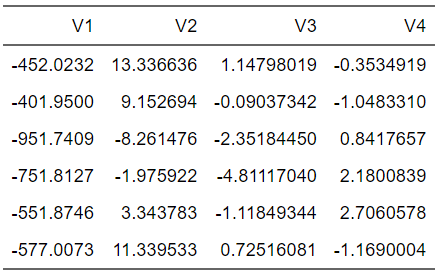
\includegraphics[width=\textwidth]{IMG/T2.png}
		\caption{Base de datos centrada y proyectada sobre los vectores propios (primeros 5 casos).}
		\label{fig:f4}
	\end{minipage}\hfill
\end{figure}

Se observa como los valores más grandes de los valores proyectados se encuentran entre las componentes 1 y 2.

\newpage

\subsection{Proyección en 1D}

Debido al sorprendente resultado que indica que el 99\% de la variabilidad de los datos recae sobre la primer componente, se decidió probar a graficar la primer componente en un gráfico de puntos unidimensional. El resultado fue el siguiente:

\begin{figure}[h!]
	\centering
	\begin{minipage}{1.1\textwidth}
		\centering
		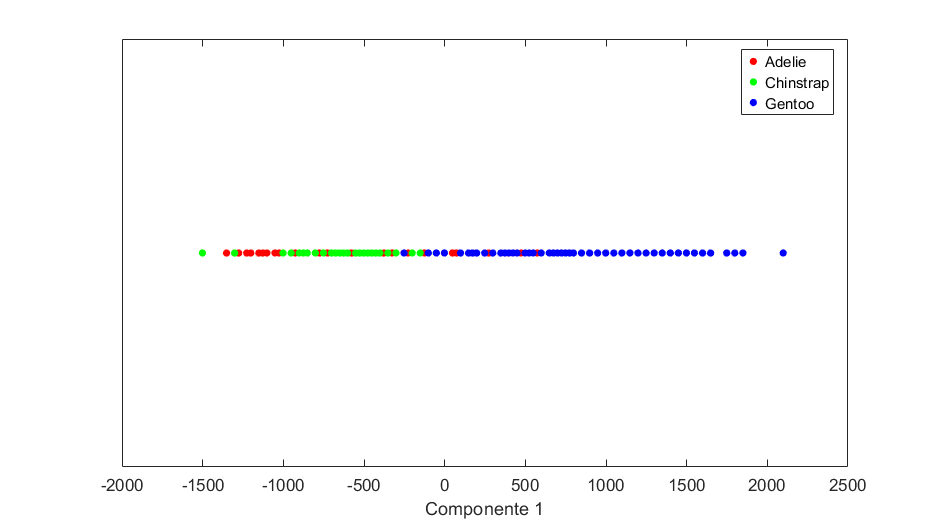
\includegraphics[width=\textwidth]{IMG/G3.png}
		\caption{Proyección en 1D sobre el componente 1.}
		\label{fig:f5}
	\end{minipage}\hfill
\end{figure}

El gráfico muestra la proyección de los datos en un espacio unidimensional, donde se observa que la mitad derecha esta mayormente representada por pingüinos de la especie Gentoo, mientras que la mitad izquierda presenta el problema del traslape entre clases. Pese a que la varianza explicada sea del 99\%, no se puede interpretar mucho a simple vista.

\newpage

\subsection{Proyección en 2D}

\begin{figure}[h!]
	\centering
	\begin{minipage}{1.1\textwidth}
		\centering
		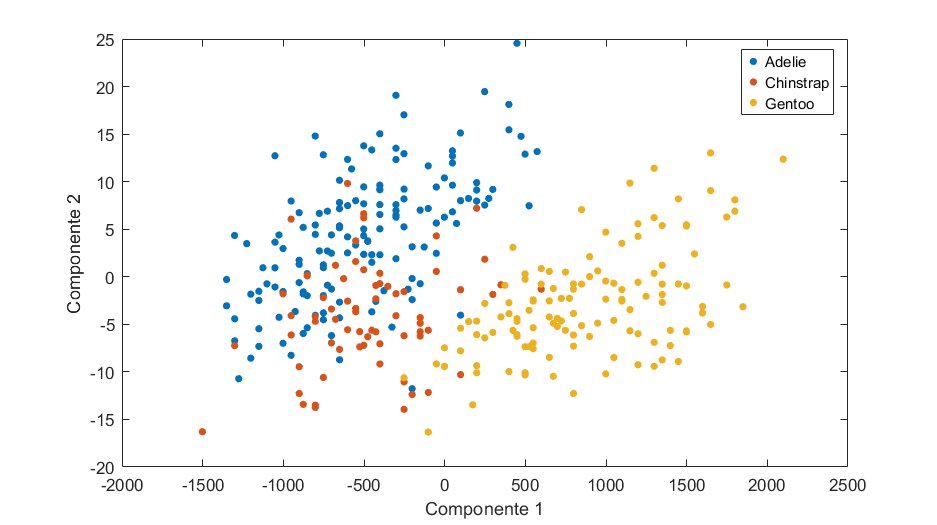
\includegraphics[width=\textwidth]{IMG/G4.png}
		\caption{Proyección en 2D sobre el componente 1 y 2.}
		\label{fig:f6}
	\end{minipage}\hfill
\end{figure}

El resultado obtenido captura mejor la esencia de los datos y nos permite observar el fuerte traslape que existe entre la especie Adelie y Chinstrap en las nubes de puntos de los datos, existiendo también un ligero traslape de los Chinstrap con los gentoo.

\newpage

\subsection{Proyección en 3D}

\begin{figure}[h!]
	\centering
	\begin{minipage}{1.1\textwidth}
		\centering
		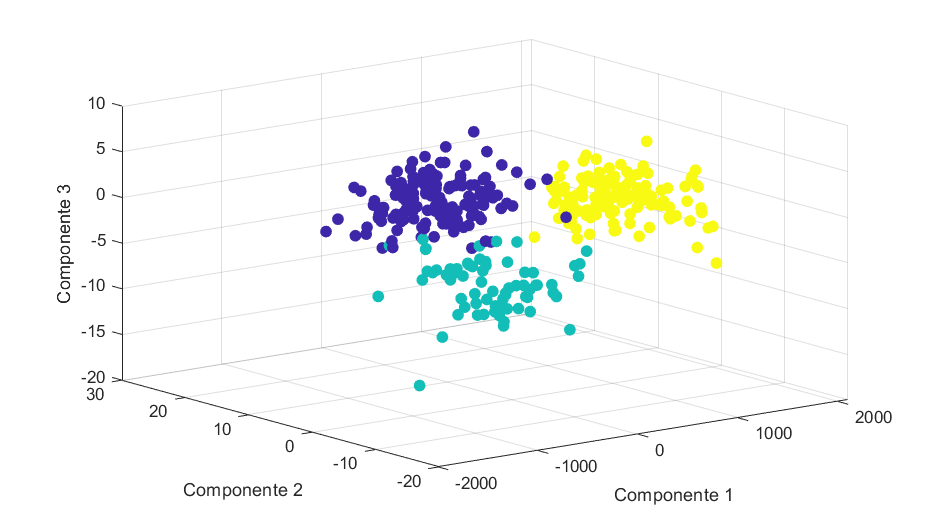
\includegraphics[width=\textwidth]{IMG/G5.png}
		\caption{Proyección en 3D sobre el componente 1, 2 y 3.}
		\label{fig:f7}
	\end{minipage}\hfill
\end{figure}

Al usar las primeras 3 componentes para proyectar los datos en un espacio de 3 dimensiones, se logra apreciar mejor la separación de los datos en 3 nubes de puntos que se encuentran mejor diferenciadas en comparación con las representaciones anteriores, aquí se observa un menor traslape entre las clases problemáticas de Adelie y Chinstrap. 


\newpage
	
\section{Conclusiones}
	
Después de realizar el ejercicio de explorar una base de datos y aplicarle PCA para poder proyectar su información concentrada en un espacio de menor dimensionalidad, se pudo observar como el PCA mejora sustancialmente la representación de los datos al poder comprimir las variables en un espacio de menor dimensionalidad sin perder apenas información.

La técnica es eficaz, relativamente simple y bastante potente, aunque presenta algunas debilidades. Una de las principales es su sensibilidad a la escala de las variables. Como se observó en el ejercicio, la variable masa corporal, que tenía los valores más grandes, resultó ser la que más aportó a la primera componente principal. Esto se debe a que, al tener mayor variabilidad absoluta, influye más en el cálculo de los valores propios, lo que provoca que se le atribuya una mayor capacidad explicativa. Para enfrentar este tipo de situaciones, se recomienda estandarizar los datos mediante una transformación $Z$, o bien utilizar la matriz de correlaciones en lugar de la matriz de covarianzas.

El otro problema que acarrea consigo el PCA es la posibilidad de que la matriz de varianzas y covarianzas o la de correlaciones (cualquiera que se este usando) tenga la particularidad de ser NO invertible, por lo que ahí la técnica ya no es posible aplicarla.

Más allá de estos problemas, la técnica probo ser buena para mejorar la visualización de los datos para este caso de aplicación.

\newpage

	
\section{Referencias}  % Sección numerada de referencias
\bibliographystyle{apalike}  % Estilo de citas (puedes cambiarlo)
\bibliography{Biblio}        % Nombre del archivo BibTeX (sin extensión)

\newpage
	
\section{Anexos}	
\subsection{Implementación de la exploración y el PCA en MATLAB}
\begin{minted}[linenos,firstnumber=1]{matlab}
%% Cargar la base de datos en formato CSV %%
ruta = "penguins.csv";
datos = readtable(ruta); % Leer el archivo CSV en una tabla
size(datos); % Ver el tamaño de los datos

% 1 etiqueta de clasificación (Species)
% 3 características categóricas (Isla, sexo y año de observación)
% 4 variables continuas: bill length, bill depth, fliper y bodymass

% Filtrar solo las columnas numéricas y eliminar filas con datos faltantes
indices = find(any(isnan(datos{:, 4:7}), 2)); % Buscar filas con valores NaN en las columnas 4 a 7
datos1 = datos;
datos1(indices, :) = []; % Eliminar esas filas

% Extraer las variables numéricas y la especie para el gráfico
% Extraer las variables numéricas y la especie para el gráfico
especie = datos1.species; % Columna 'species' con las etiquetas de especies
% Convertir la columna 'especie' en un vector de tipo categorical
especie = categorical(especie); % Convertir a tipo categorical, que gscatter entiende
datos1 = table2array(datos1(:, 4:7)); % Convertir las columnas 4 a 7 a un arreglo numérico

%% Gráficos descriptivos %%
% Graficar el gráfico de dispersión usando gscatter
% Longitud del pico y ancho del pico
subplot(2,2,1)
gscatter(datos1(:,1), datos1(:,2), especie,"filled"); 
xlabel('Longitud del pico'); % Etiqueta del eje x
ylabel('Profundidad del pico'); % Etiqueta del eje y
title('G1'); % Título del gráfico

% Longitud del pico y longitud de la aleta %
subplot(2,2,2)
gscatter(datos1(:,1), datos1(:,3), especie,"filled");
xlabel('Longitud del pico'); % Etiqueta del eje x
ylabel('Longitud de la aleta'); % Etiqueta del eje y
title('G2'); % Título del gráfico
% Longitud del pico y masa corporal
subplot(2,2,3)
gscatter(datos1(:,1), datos1(:,4), especie,"filled");
xlabel('Longitud del pico'); % Etiqueta del eje x
ylabel('Masa corporal'); % Etiqueta del eje y
title('G3'); % Título del gráfico
% Ancho del pico y Longitud de la aleta
subplot(2,2,4)
gscatter(datos1(:,2), datos1(:,3), especie,"filled");
xlabel('Profundidad del pico'); % Etiqueta del eje x
ylabel('Longitud de la aleta'); % Etiqueta del eje y
title('G4'); % Título del gráfico

%% Exploración en 3D %&
% Crear un gráfico 3D
subplot(1,2,1)
scatter3(datos1(:,1), datos1(:,2), datos1(:,3), 50, especie, 'filled'); 
% Ajustar etiquetas y título
xlabel('Longitud del pico');
ylabel('Profundidad del pico');
zlabel('Longitud del aletín');
title('');

subplot(1,2,2)
scatter3(datos1(:,2), datos1(:,3), datos1(:,4), 50, especie, 'filled'); 
% Ajustar etiquetas y título
xlabel('Profundidad del pico');
ylabel('Largo de la aleta');
zlabel('Masa corporal');
title('');
% Mostrar la leyenda de colores
% Guardar como archivo PNG

%% HACER EL PCA %%

% Obtener la media de los datos
%% Cambio de coordenadas %%
medias = mean(datos1)
cdatos = datos1 - medias % Centrar en la media


% Calculo de la covarianza %
n = size(datos1);
Si = (cdatos'*cdatos)/(n(1)-1)

%% Calcular los eigen valores %%
[V, D] = eig(Si)

100*diag(D)/sum(diag(D))

%% Calcular los scores %%
%% Calcular los scores %%
NB = cdatos * V; % Proyección de los datos

% Crear una dispersión en 1D (todos los puntos con la misma Y)
y = zeros(size(NB, 1), 1); % Todos los puntos en Y=0
gscatter(NB(:,4), y, especie, 'rgb', '.', 15);
xlabel('Componente 1');
yticks([]); % Eliminar marcas del eje Y
ylabel('');
title('Proyección 1D sobre el componente 1');

%% Gráfico en 2d con la primer y segunda componente %%
gscatter(NB(:,4), NB(:,3), especie,"filled");
xlabel('Componente 1'); % Etiqueta del eje x
ylabel('Componente 2'); % Etiqueta del eje y
title(''); % Título del gráfico

%% Crear un gráfico 3D %%
scatter3(NB(:,4), NB(:,3), NB(:,2), 50, especie, 'filled'); 
% Ajustar etiquetas y título
xlabel('Componente 1');
ylabel('Componente 2');
zlabel('Componente 3');
title('');
\end{minted}
	
	
	
	
\end{document}

